\documentclass{beamer}
\usetheme{metropolis}
\usepackage{graphicx}
\usepackage{subfig}
\usepackage{tcolorbox}
\title{Computer Logic and Digital Circuit Design (PHYS306/COSC330): Unit 1.3}
\author{Jordan Hanson}
\institute{Whittier College Department of Physics and Astronomy}

\begin{document}
\maketitle

\section{Summary}

\begin{frame}{Unit 1.3 Summary - Working with Binary}
\textbf{Reading: Digital Fundamentals (DF) Ch. 2 (see Moodle)}
\begin{enumerate}
\item Number representation
\item Binary conversions
\item Binary arithmetic
\item The floating-point system
\item Hexadecimals, Binary-Coded Decimals (BCD), Gray codes, and ASCII
\end{enumerate}
\textbf{Homework: exercises 5-16, 19-32, 35-38, 45, 53, 58 Ch. 2 (DF) (two weeks).}
\end{frame}

\section{Number representation}

\begin{frame}{Number representation}
Questions:
\begin{itemize}
\item A simple question: how many students do we have in this class? \\
\item Una simple pregunta: ?`Cu\'{a}ntos estudiantes tenemos en esta clase? \\
\item Une question simple: Combien d'\'{e}tudiants est-ce que nous avons dans cette classe?
\end{itemize}
What languages do computers speak?  How can we store and transmit numbers through circuits?  (We cannot use voltage magnitudes).
\end{frame}

\begin{frame}{Number representation}
\textbf{Consider the number \alert{37}} \\ \vspace{1cm}
\begin{columns}[T]
\begin{column}{0.5\textwidth}
\centering
Numbers \\
\hrulefill
\begin{itemize}
\item 0d37
\item 0b100101
\item 0x25
\end{itemize}
\end{column}
\begin{column}{0.5\textwidth}
\centering
Expanded notation \\
\hrulefill
\begin{itemize}
\item $3\times 10^1 + 7 \times 10^0$
\item $1\times 2^5 + 1 \times 2^2 + 1 \times 2^0$
\item $2\times 16^1 + 5 \times 16^0$
\end{itemize}
\end{column}
\end{columns}
\end{frame}

\begin{frame}{Number representation}
\textbf{Consider the number \alert{412}} \\ \vspace{1cm}
\begin{columns}[T]
\begin{column}{0.5\textwidth}
\centering
Numbers \\
\hrulefill
\begin{itemize}
\item 0d412
\item 0b110011100
\item 0x100
\end{itemize}
\end{column}
\begin{column}{0.5\textwidth}
\centering
Expanded notation \\
\hrulefill
\begin{itemize}
\item $4\times 10^2 + 1\times 10^1 + 2\times 10^0$
\item $1\times 2^8 + 1\times 2^7 + 1\times 2^4 + 1\times 2^3 + 1\times 2^2$
\item $1\times 16^2$
\end{itemize}
\end{column}
\end{columns}
\end{frame}

\begin{frame}{Number representation}
\textbf{Number representations} - Digits, weights, and a common base \\ \vspace{1cm}
\begin{columns}[T]
\begin{column}{0.5\textwidth}
\centering
\begin{itemize}
\small
\item A number is written with \textbf{digits} that have \textbf{weights}.
\item A \textbf{weight} is a power of a \textbf{base}.
\item At right, the \textbf{base} is ten, and the \textbf{weights} are $10^2$, $10^1$, and $10^0$.
\item The \textbf{digits} are four, one, and two.
\item The digits cannot represent numbers larger than the base.
\end{itemize}
\end{column}
\begin{column}{0.5\textwidth}
\centering
Expanded notation \\
\hrulefill
\begin{itemize}
\item $412 = 4\times 10^2 + 1\times 10^1 + 2\times 10^0$
\end{itemize}
\end{column}
\end{columns}
\end{frame}

\begin{frame}{Number representation}
\textbf{Number representations} - (Aside) please use scientific notation, and here is why: \alert{digit minimization!} \\ \vspace{1cm}
\begin{columns}[T]
\begin{column}{0.5\textwidth}
\centering
\begin{itemize}
\small
\item Scientific notation \textbf{factors the largest weight}.
\item Results in weights that are less than one.
\item Weights that are less than one go to the right of the \textbf{decimal point}.
\item Return here with \textit{floating-point} representation.
\end{itemize}
\end{column}
\begin{column}{0.5\textwidth}
\centering
Expanded notation \\
\hrulefill
\begin{itemize}
\item $412,000,000 = 4\times 10^8 + 1\times 10^7 + 2\times 10^6 + 0\times 10^5 + 0\times 10^4 + 0\times 10^3 + 0\times 10^2 + 0\times 10^1 + 0\times 10^0$
\item $412,000,000 = 4.12 \times 10^8 = (4\times 10^0 + 1\times 10^{-1} + 2\times 10^{-2}) \times 10^8$
\end{itemize}
\end{column}
\end{columns}
\end{frame}

\begin{frame}{Number representation}
\textbf{Number representations} - (Aside) please use scientific notation, and here is why: \alert{arithmetic operations with large numbers!} \\ \vspace{1cm}
\begin{enumerate}
\item $4200 \times 4200 = (4.2 \times 10^{3})^2 = (4.2)^2 \times 10^6 \approx 16 \times 10^6$
\item $\approx 17.6 \times 10^6$ if you account for the $0.2$ ...
\end{enumerate}
\hrulefill
\begin{enumerate}
\item $4000/3000 = 4 \times 10^{3} \times \frac{1}{3} \times 10^{-3} = \frac{4}{3}$
\item $\frac{4}{3} \approx 1.33$
\end{enumerate}
\end{frame}

\begin{frame}{Number representation}
Expand the following numbers to expanded decimal notation:
\begin{itemize}
\item -10.432
\item 800,000,144
\end{itemize}
Expand the following numbers to expanded binary notation:
\begin{itemize}
\item 10011010
\item 11110000
\end{itemize}
Convert the following decimal numbers to binary notation:
\begin{itemize}
\item 260
\item 560
\end{itemize}
\textbf{Volunteer to board?} - Key is explaining how you did the binary conversions
\end{frame}

\section{Binary Conversion}

\begin{frame}{Binary Conversion}
How did you do the conversions to binary?  Is there a systematic what to do this? \\
\begin{itemize}
\item \textit{Successive Approximation} - like a number puzzle (\textit{Sum of Weights Method})
\item \textit{Successive Division Method} - Example of an algorithm
\end{itemize}
\hrulefill \\ \vspace{0.5cm}
\textit{Successive approximation} technique (does this remind you of doing division in your head?)
$260$...$2^8 = 256$.  Now we need four more...$4 = 2^2$.  So $2^8 + 2^2 = 0b10000100$ \\ \vspace{0.5cm}
What is 328 divided by 3?  Ok try 100 because three times one hundred is close...
\end{frame}

\begin{frame}{Binary Conversion}
\textit{Successive Division Method} \\ \vspace{0.5cm} \hrulefill \\
$0d412 = 0b110011100 = 2^8 + 2^7 + 2^4 + 2^3 + 2^2$ \\
Algorithm:
\begin{enumerate}
\item Divide the decimal number by 2, and write down the remainder.  This is the \textit{least-significant bit} or LSB.
\item Keep dividing and recording the remainders in order, until you reach a dividend of 1.
\item $1/2 = 0 r 1$, so the \textit{most-significant bit}, or MSB, is always 1.
\end{enumerate}
Convert 412 to binary using the successive division method.
\end{frame}

\begin{frame}{Binary Conversion}
Convert the numbers at right to binary. \\ \vspace{1cm}
\begin{columns}[T]
\begin{column}{0.5\textwidth}
\begin{itemize}
\item $2^0 = 1$
\item $2^1 = 2$
\item $2^2 = 4$
\item $2^3 = 8$
\item $2^4 = 16$
\item $2^5 = 32$
\item $2^6 = 64$
\item $2^7 = 128$
\end{itemize}
\end{column}
\begin{column}{0.5\textwidth}
\begin{enumerate}
\item 93
\item 189
\item 270
\end{enumerate}
\textit{Note: how many bits do you need for that last one?}  For binary, show that the highest representable number with $n$ bits is $2^n-1$.
\end{column}
\end{columns}
\end{frame}

\begin{frame}{Binary Conversion}
In decimal notation, we represent numbers $\in [0-1]$ with digits to the right of the \textit{decimal point.} \\ \vspace{0.5cm}
In expanded notation: \\
$42.42 = 4\times 10^{1} + 2\times 10^{0} ~~ . ~~ 4\times 10^{-1} + 2\times 10^{-2}$ \\ \vspace{0.5cm}
We have a similar notation in other number systems: \\
$101.11 = 2^2 + 2^0 ~~ . ~~ 2^{-1} + 2^{-2}$
\end{frame}

\begin{frame}{Binary Conversion}
\textit{Successive Multiplication Method} \\ \vspace{0.5cm} \hrulefill \\
$0d0.48 = 0b0.011110101 = 2^{-2}+2^{-3}+2^{-4}+2^{-5}+2^{-7}+2^{-9}$ \\
Algorithm:
\begin{enumerate}
\item Multiply the decimal fraction by 2, and write down the \textit{carry} (the 1 to the left of the decimal point, else 0).  This is the \textit{most-significant bit} or MSB.
\item Keep multiplying and recording the carries in order, to the desired precision.
\item Watch for repeating patterns.
\end{enumerate}
Convert 0.48 to binary using the successive multiplication method until you identify a repeating pattern.
\end{frame}

\section{Binary Arithmetic}

\begin{frame}{Binary Arithmetic}
Binary arithmetic, like decimal arithmetic, relies upon \textit{carries} and \textit{borrows}.  For example in decimal: \\ \vspace{0.5cm}
\begin{itemize}
\item $8+7 = 5 c 1 = 15$
\item $3+4 = 7 c 0 = 7$
\item $8-2 = 6 b 0 = 6$
\item $10-5 = (0 b 10) - 5 = 5$
\item $13-7 = (0 b 10) - 4 = 6$ 
\end{itemize}
\end{frame}

\begin{frame}{Binary Arithmetic}
In binary there are limited combinations, so we may form a set of addition and subtraction rules that describe all possibilities: \\ \vspace{0.5cm}
\hrulefill
\begin{columns}[T]
\begin{column}{0.5\textwidth}
\begin{itemize}
\item $0+0=0$
\item $1+0=1$
\item $0+1=1$
\item $1+1 = 0 c 1$
\end{itemize}
\end{column}
\begin{column}{0.5\textwidth}
\begin{itemize}
\item $0-0=0$
\item $1-0=1$
\item $0-1=0b1$
\item $1-1 = 0$
\end{itemize}
\end{column}
\end{columns}
\tiny
In the fourth rule for the addition set, the carry works the same way as a decimal carry: we add that $1$ to the digit corresponding to the next power of 2.  Similarly, in the third rule of the subtraction set, we subtract the $1$ on the left side of the equation from a $1$ from the digit corresponding to the next highest power of 2 available.
\end{frame}

\begin{frame}{Binary Arithmetic}
Complete the following additions and subtractions: \\ \vspace{0.5cm}
\hrulefill
\begin{columns}[T]
\begin{column}{0.5\textwidth}
\begin{itemize}
\item $10+11$
\item $111+1$
\item $111+111$
\item $1010+101$
\end{itemize}
\end{column}
\begin{column}{0.5\textwidth}
\begin{itemize}
\item $10-11$
\item $111-1$
\item $111-111$
\item $1010-101$
\end{itemize}
\end{column}
\end{columns}
\end{frame}

\begin{frame}{Binary Arithmetic}
Binary multiplication stems from another set of rules: \\ \vspace{0.5cm}
\hrulefill
\begin{columns}[T]
\begin{column}{0.5\textwidth}
\begin{itemize}
\item $0\times 0=0$
\item $1\times 0=0$
\item $0\times 1=0$
\item $1\times 1=1$
\end{itemize}
\end{column}
\begin{column}{0.5\textwidth}
\small
Binary division is exactly the same as decimal long division.  Let's work these examples on the board:
\begin{itemize}
\item 145/12
\item 1101/101
\item 45/3
\item 111/10
\end{itemize}
\end{column}
\end{columns}
\small
Of what logic operation does binary multiplication remind you?
\end{frame}

\begin{frame}{Binary Arithmetic}
We need a few tools to improve our arithmetic techniques in order to install these functions into circuits.  Consider two actions:
\begin{itemize}
\item NOT to the bit sequence of a number: \textbf{\alert{1's compliment}}
\item Add 1 to the 1's compliment: \textbf{\alert{2's compliment}}
\end{itemize}
\end{frame}

\begin{frame}{Binary Arithmetic}
Logical operator representation of these actions for 8-bits: \\ \vspace{0.5cm}
\hrulefill
\begin{columns}[T]
\begin{column}{0.5\textwidth}
\begin{figure}
\centering
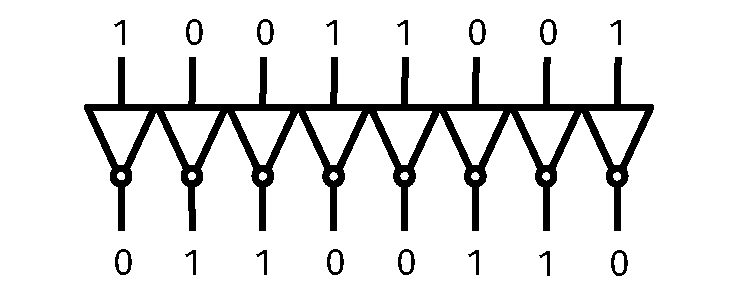
\includegraphics[width=\textwidth]{figures/1Compliment.pdf}
\caption{\label{fig:1comp} Representation of 1's compliment.}
\end{figure}
\end{column}
\begin{column}{0.5\textwidth}
\begin{figure}
\centering
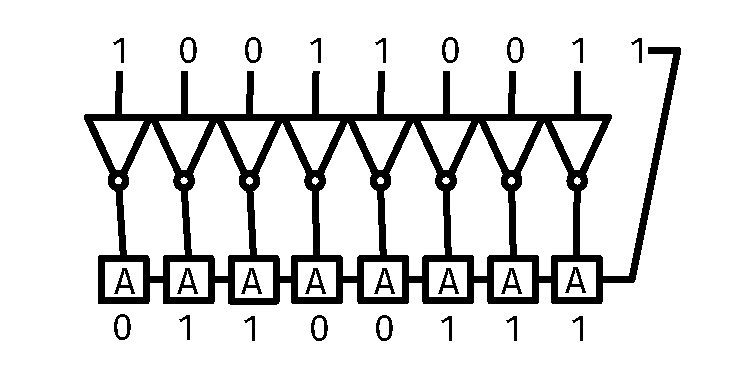
\includegraphics[width=\textwidth]{figures/2Compliment.pdf}
\caption{\label{fig:2comp} Representation of 2's compliment.}
\end{figure}
\end{column}
\end{columns}
\end{frame}

\begin{frame}{Binary Arithmetic}
Exercises, and a realization for the purpose of 2's compliment. \\ \vspace{0.5cm}
\hrulefill
\begin{columns}[T]
\begin{column}{0.33\textwidth}
Take the 1's compliment of the right-hand number, and complete the addition:
\begin{itemize}
\item $111+(000)$
\item $111+(111)$
\end{itemize}
\end{column}
\begin{column}{0.33\textwidth}
Take the 2's compliment of the right-hand number, and complete the addition:
\begin{itemize}
\item $111+(000)$
\item $111+(111)$
\end{itemize}
\end{column}
\begin{column}{0.33\textwidth}
Same, \alert{but drop the MSB}:
\begin{itemize}
\item $1010+(1010)$
\item $1100+(1100)$
\end{itemize}
\end{column}
\end{columns}
\vspace{0.5cm}
\small
For what purpose are we going to use the 2's compliment?
\end{frame}

\begin{frame}{Binary Arithmetic}
The answer: representing negative numbers.  For \textit{2's compliment form signed binary numbers, the MSB is the \textbf{sign bit}}.  To convert to decimal, \alert{give the MSB a negative weight}: \\ \vspace{0.5cm}
Example: $10101010$ \\ 
This is a negative number because the MSB is a $1$.  Converting in expanded form: $-2^7+2^5+2^3+2^1 = -128+32+8+2 = -86$.
\end{frame}

\begin{frame}{Binary Arithmetic}
Consider the effect on the maximum \textit{range} of binary numbers after sacrificing the MSB to flag numbers less than zero.  For 8-bits unsigned numbers, the range is [0-255]: \\ \vspace{0.5cm}
\begin{table}
\small
\centering
\begin{tabular}{c c c c}
$n$-bits & 8 & 16 \\
Lowest unsigned & 0 & 0 \\
Highest unsigned & 255 & 65535 \\
Lowest signed & -128 & -32768 \\
Highest signed & 127 & 32767
\end{tabular}
\caption{\label{tab:ranges} The ranges of unsigned and signed numbers using $n$ digits.}
\end{table}
\small
By changing the role of the MSB, we are not reducing the \textit{range} of numbers, just its \textit{location}.  Related to \textit{conservation of information...}
\end{frame}

\begin{frame}{Binary Arithmetic}
2's compliment, signed number representation and conversion, arithmetic with negative numbers \\ 
\hrulefill
\begin{enumerate}
\item Write -278 in binary, 2's compliment form.
\item Convert -302 and 65 each to binary, and add them.
\item This number is in 2's compliment form: 11001101.  Convert it to decimal. 
\end{enumerate}
\end{frame}

\section{The Floating-Point System}

\begin{frame}{The Floating-Point System}
\alert{Who has taken software programming?}\footnote{Normally, this is a pre-requisite for this course, but in this innaugural year we are more flexible.}\\
In software code, we allocate memory for variables which could be decimal numbers.  In C++, this might look like \\ \vspace{0.5cm}
\textit{\textbf{float} var = } $15.237$; \\ \vspace{0.15cm}
\textit{\textbf{double} var = } $1.61E-19$; \\ \vspace{0.15cm}
\textit{\textbf{unsigned int} var = } $8$; \\ \vspace{0.15cm}
\textit{\textbf{long int} var = } $3200000000$; \\ \vspace{0.15cm}
We will now learn the origin and purpose of these keywords.
\end{frame}

\begin{frame}{The Floating-Point System}
A \textit{floating-point number} is a general system for storage of wide ranges of real numbers in binary.  \alert{The structure of a floating-point number:} \\ \vspace{0.125cm}
\tiny
\begin{table}
\centering
\begin{tabular}{| c | c | c | c | c | c |}
\hline
N & Binary & Scientific Notation & \alert{Sign bit} & \alert{Exponent} & \alert{Mantissa} \\ \hline
$-10.23$ & $-1010.0011101$ & $-1.0100011101 \times 2^{3}$ & 1 & 10000010 & 01000111010000000000000 \\ \hline
$22.3$ & $10110.01001100$ & $1.011001001100 \times 2^{4}$ & 0 & 10000011 & 01100100110000000000000 \\ \hline
\end{tabular}
\caption{\label{tab:floats} \small For \textbf{float} or \textbf{single} precision, the number of bits allowed for the sign, exponent and mantissa is \textbf{32}.  The exponent is $3+127$ in binary.  We \textit{bias} the exponent by 127 so that the range of exponents can be both negative and positive.}
\end{table}
\small
\begin{itemize}
\item Float or single precision: 32 bits
\item Double precision: 64 bits
\end{itemize}
\end{frame}

\begin{frame}{The Floating-Point System}
\alert{The structure of a floating-point number:} \\ \vspace{0.125cm}
\tiny
\begin{table}
\centering
\begin{tabular}{| c | c | c | c | c | c |}
\hline
N & Binary & Scientific Notation & \alert{Sign bit} & \alert{Exponent} & \alert{Mantissa} \\ \hline
$22.3$ & $10110.01001100$ & $1.011001001100 \times 2^{4}$ & 0 & 10000011 & 01100100110000000000000 \\ \hline
$6.825$ & $1010.11010011$ & $1.01011010011 \times 2^{3}$ & 0 & 10000010 & 01011010011000000000000 \\ \hline
\end{tabular}
\caption{\label{tab:floats2} \small Note that the MSB in scientific notation is \textbf{dropped} in the mantissa.  Why?}
\end{table}
\small
Convert the following numbers into \textbf{floats}:
\begin{itemize}
\item 8.125
\item -4.0625
\end{itemize}
\end{frame}

\begin{frame}{The Floating-Point System}
\small
\textbf{Addition and subtraction with signed numbers}: either number can be positive/negative, and the larger/smaller number by magnitude.  Thus, 4 combinations are possible:
\begin{table}
\centering
\begin{tabular}{| c | c | c |}
\hline
... & Negative & Positive \\ \hline
Larger & A & B \\ \hline
Smaller & C & D \\ \hline
\end{tabular}
\caption{\label{tab:floats3} Four categories, two numbers, so 6 initial pairs: AB AC AD BC BD CD.  However, AB and CD aren't real choices, so the list is: AC AD BC BD.}
\end{table}
Bottom line: both negative, both positive, one negative one positive (two cases)
\end{frame}

\begin{frame}{The Floating-Point System}
The results:
\begin{enumerate}
\item Both negative $\rightarrow$ \alert{discard the carry}
\item One positive, one negative, and the negative number has a larger magnitude
\item One positive, one negative, and the positive number has a larger magnitude $\rightarrow$ \alert{discard the carry}
\item Both positive
\end{enumerate}
\end{frame}

\begin{frame}{The Floating-Point System}
\small
\textbf{Example of negative-negative case:} $-13-9=-22$. \\ \vspace{0.5cm}
\begin{enumerate}
\item Identify case: both are negative, with magnitudes of 13 and 9.
\item Decide $n$-bits.  Ensure that $2^n-1$ is much larger than other numbers.  Let's choose $n=8$.
\item Convert the first magnitude (13) to 2's compliment form: $2s(00001101) = 11110011$
\item Convert the second magnitude (9) to 2's compliment form: $2s(00001001) = 11110111$
\item Add them, and in this case, drop the final carry: $11101010$
\item Check: $2s(11101010) = 00010110 = 22$
\end{enumerate}
\end{frame}

\section{Hexadecimals, BCD, Gray-Codes, and ASCII}

\begin{frame}{Hexadecimals, BCD, Gray-Codes, and ASCII}
Why do we use Hexadecimals? \\ \vspace{0.5cm}
\url{https://youtu.be/DqfnMzDhi38} \\
In case you get your butt stranded on Mars, and need to devise a rag-tag communication system from a camera-pole, is why.
\end{frame}

\begin{frame}{Hexadecimals, BCD, Gray-Codes, and ASCII}
\small
Astronaut Watney needs a way to cram more information into shorter-length words...hexadecimals
\tiny
\begin{table}
\centering
\begin{tabular}{c c c}
Decimal & Binary & Hexadecimal \\ 
0 & 0000 & 0 \\
1 & 0001 & 1 \\
2 & 0010 & 2 \\
3 & 0011 & 3 \\
4 & 0100 & 4 \\
5 & 0101 & 5 \\
6 & 0110 & 6 \\
7 & 1111 & 7 \\
8 & 1000 & 8 \\
9 & 1001 & 9 \\
10 & 1010 & A \\
11 & 1011 & B \\
12 & 1100 & C \\
13 & 1101 & D \\
14 & 1110 & E \\
15 & 1111 & F 
\end{tabular}
\caption{\small \label{tab:hex1} Decimal, binary and Hexadecimal representations of numbers.  What do you notice that is different between the representations?}
\end{table}
\end{frame}

\begin{frame}{Hexadecimals, BCD, Gray-Codes, and ASCII}
\small Because $2^4 = 16$, we may group bits in bit sequences in groups of four, and read out the hexadecimal conversion: \\ \vspace{0.5cm}
$0b11010010 = 1101~0010 = (13)~(2) = 0xD2$ \\ \vspace{0.5cm}
On page 71 of DF: ``It should be clear that it is much easier to deal with a hexadecimal number than with the equivalent binary number.  Since conversion is so easy, the hexadecimal system is widely used for representing binary numbers in programming, printouts, and displays.'' \\ \vspace{0.5cm}
\alert{It is probably important.}  What follows is a few examples of how I've encountered hexadecimals.
\end{frame}

\begin{frame}[fragile]{Hexadecimals, BCD, Gray-Codes, and ASCII}
\tiny
\begin{verbatim}
set key at 500,73 box on samplen 2 spacing 1.5 font "Courier,16" width 2
set xrange [1:1e3]
set yrange [0:180]
set format x "10^{%T}"
set rmargin 8
set lmargin 13
set tmargin 2
set bmargin 6
set xlabel "Frequency [MHz]" font "Courier,28" offset 0,-2,0
set ylabel "Phase (deg)" font "Courier,28" offset -5,0,0
set ytics scale 2 font "Courier,28"
set xtics scale 2 font "Courier,28" offset 0,-1,0
set style line 6 linecolor rgb "#000000" linewidth 5.000 dashtype 3 pointtype 2
set style line 7 linecolor rgb "#BBBBBB" linewidth 5.000 dashtype 3 pointtype 2
set linestyle 1 lc rgb "#000000" lw 5
set linestyle 2 lc rgb "#444444" lw 5
set linestyle 3 lc rgb "#888888" lw 5
set linestyle 4 lc rgb "#BBBBBB" lw 5
set linestyle 5 lc rgb "#DDDDDD" lw 5
set terminal postscript color enhance
\end{verbatim}
\end{frame}

\begin{frame}{Hexadecimals, BCD, Gray-Codes, and ASCII}
\begin{figure}
\centering
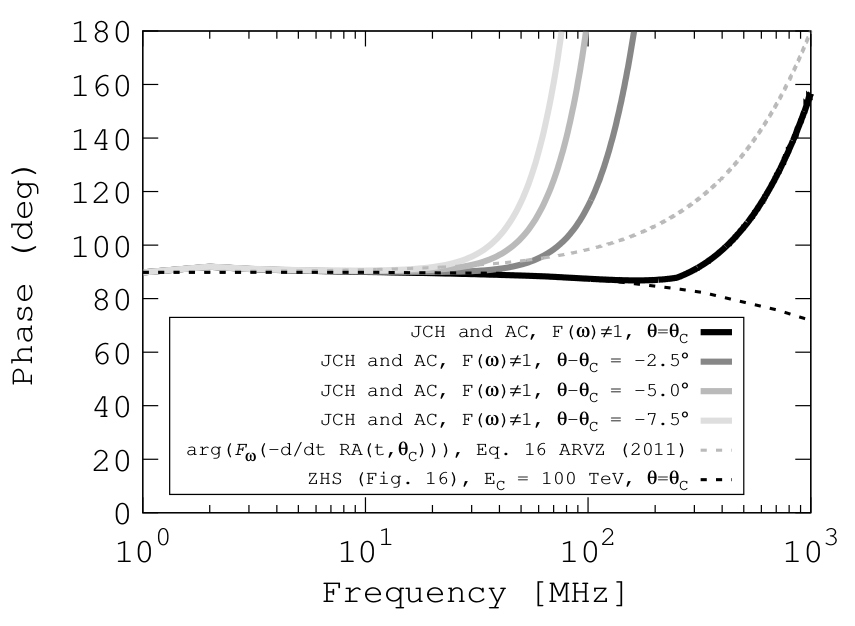
\includegraphics[width=0.75\textwidth]{figures/fromPaper.png}
\caption{\label{fig:frompaper} A figure from a recent paper we published about neutrino signals in ice.  The hexadecimals were used to encode the line-colors.}
\end{figure}
\end{frame}

\begin{frame}{Hexadecimals, BCD, Gray-Codes, and ASCII}
\textbf{A math problem:} If the RGB (red, green, blue) codes have the following format 0xA1B2C3, where each hex word (two characters) represents an amount of red, green, and blue (sequentially), how many distinct shades of each are technically possibe? How many colors are therefore possible (even if a standard monitor could not resolve them)? \\ \vspace{0.5cm}
\textbf{Volunteer to board?}
\end{frame}

\begin{frame}{Hexadecimals, BCD, Gray-Codes, and ASCII}
\small In graduate school, I was responsible for designing and deploying a housekeeping integrate circuit (HK board).  The task of this device was to control which subsystems are activated in an ARIANNA station, managing power consumption.
\begin{figure}
\centering
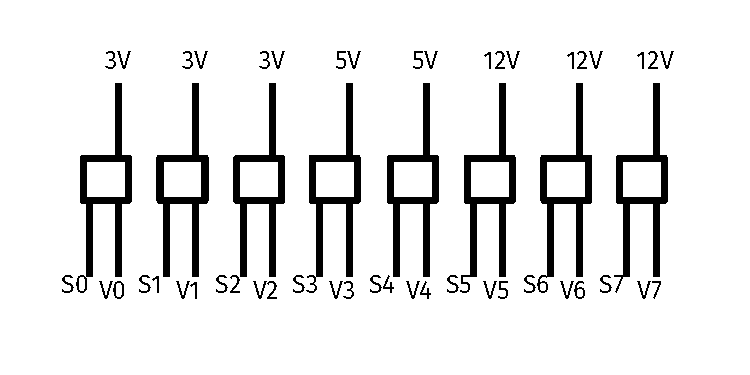
\includegraphics[width=0.75\textwidth,trim=0cm 1cm 0cm 0.5cm,clip=true]{figures/RelayBank.pdf}
\caption{\label{fig:relay} \small Symbolic representation of a relay bank. \textit{Raising} the various signals $S_{\rm i}$ to a HIGH state connects the sub-system voltages $V_{\rm i}$ to power sources at the given voltages, and setting them to LOW state powers down the subsystems.}
\end{figure}
\end{frame}

\begin{frame}{Hexadecimals, BCD, Gray-Codes, and ASCII}
\small In software, the C-code interpreted a \textit{\alert{bit-mask}} in hexadecimal, which the single-board computer (SBC) would send to the digital IO (input/output), connected to the $S_{\rm i}$ lines.  For example, $0b11100000$ activated only the 3V subsystems.
\begin{figure}
\centering
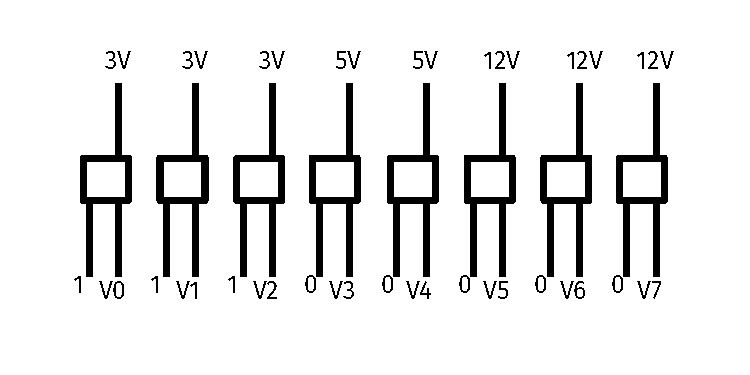
\includegraphics[width=0.75\textwidth,trim=0cm 1cm 0cm 0.5cm,clip=true]{figures/RelayBank2.pdf}
\caption{\label{fig:relay2} \small The $S_{\rm i}$ lines were controlled by the system digital IO.  The above bit-mask was sent from the C-code through the digital IO.}
\end{figure}
\end{frame}

\begin{frame}{Hexadecimals, BCD, Gray-Codes, and ASCII}
\small However, to save space on a hard drive that only had 4 GB of space, with potentially thousands of defined functions that had to send bit masks, the manufacturer designed the base bitmasking function input as a hex word (two hex characters).  In this case, it would have been $0xD0 = 0b11100000$.
\begin{figure}
\centering
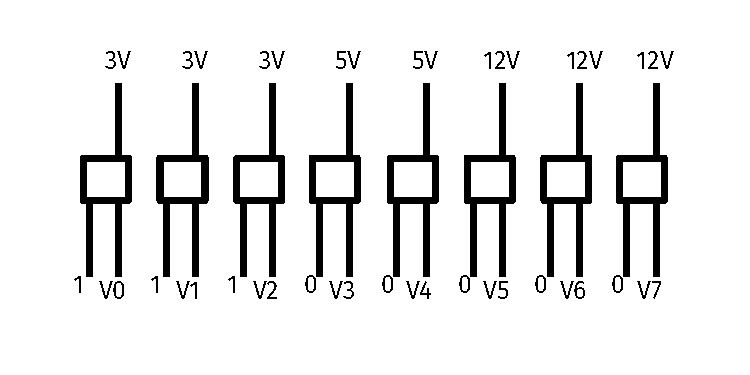
\includegraphics[width=0.75\textwidth,trim=0cm 1cm 0cm 0.5cm,clip=true]{figures/RelayBank2.pdf}
\caption{\label{fig:relay3} \small A bitmask of $D0$.}
\end{figure}
\end{frame}

\begin{frame}{Hexadecimals, BCD, Gray-Codes, and ASCII}
\begin{figure}
\centering
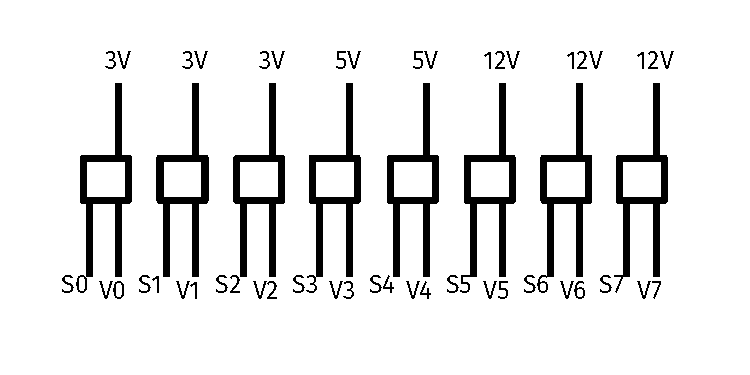
\includegraphics[width=0.75\textwidth,trim=0cm 1cm 0cm 0.5cm,clip=true]{figures/RelayBank.pdf}
\caption{\label{fig:relay4} \small The general case for the relay bank.}
\end{figure}
\small
\begin{enumerate}
\item What hex word would activate only the 5V systems?
\item What hex word would activate only the 12V sytems?
\item What hex word would activate just $S_{\rm 1}$, $S_{\rm 4}$, and $S_{\rm 7}$?
\end{enumerate}
\end{frame}

\begin{frame}{Hexadecimals, BCD, Gray-Codes, and ASCII}
\textbf{Other codings with binary and hexadecimals:}
\begin{itemize}
\item Binary coded decimals
\item Gray codes
\item ASCII
\end{itemize}
\end{frame}

\begin{frame}{Hexadecimals, BCD, Gray-Codes, and ASCII}
\small
\begin{columns}[T]
\begin{column}{0.5\textwidth}
\textbf{Binary coded decimals} (BCD): \\ \vspace{0.5cm}
The 8421 BCD system is often used in digital displays, readouts and number pads.  It combines the familiarity of decimal digits with the utility of binary. \\ \vspace{0.5cm}
For example: $0d234 = 0010~0011~0100$ in BCD.
\end{column}
\begin{column}{0.5\textwidth}
\begin{table}
\centering
\begin{tabular}{c c}
0 & 0000 \\
1 & 0001 \\
2 & 0010 \\
3 & 0011 \\
4 & 0100 \\
5 & 0101 \\
6 & 0110 \\
7 & 0111 \\
8 & 1000 \\
9 & 1001 \\
\end{tabular}
\caption{\label{tab:bcd} \small The 8421 coding for BCD.  Each four-digit bit sequence represents one decimal digit.}
\end{table}
\end{column}
\end{columns}
\end{frame}

\begin{frame}{Hexadecimals, BCD, Gray-Codes, and ASCII}
\small
\begin{columns}[T]
\begin{column}{0.5\textwidth}
\textbf{Quick exercise:} Write your first name as a decimal string ($A=1$, $B=2$, etc.) and convert it to BCD. \\ \vspace{0.5cm}
Jordan corresponds to 10 15 18 04 01 14 so 00010000 00010101 00011000 00000100 00000001 00010100
\end{column}
\begin{column}{0.5\textwidth}
\begin{table}
\centering
\begin{tabular}{c c}
Decimal digit & BCD \\
0 & 0000 \\
1 & 0001 \\
2 & 0010 \\
3 & 0011 \\
4 & 0100 \\
5 & 0101 \\
6 & 0110 \\
7 & 0111 \\
8 & 1000 \\
9 & 1001 \\
\end{tabular}
\caption{\label{tab:bcd} \small The 8421 coding for BCD.  Each four-digit bit sequence represents one decimal digit.}
\end{table}
\end{column}
\end{columns}
\end{frame}

\begin{frame}{Hexadecimals, BCD, Gray-Codes, and ASCII}
\small
\begin{columns}[T]
\begin{column}{0.5\textwidth}
\textbf{The Gray Code}: \\ \vspace{0.5cm}
The Gray code is a non-arithmetic code word system, related to binary, that minimizes transition errors by restricting one bit change per transition. \\ \vspace{0.5cm}
\textbf{Binary to Gray Code conversion}
\begin{enumerate}
\item The MSB is conserved.
\item Add consecutive binary bits starting with the MSB to obtain Gray Code bits.
\item Discard carries.
\end{enumerate}
\end{column}
\begin{column}{0.5\textwidth}
\begin{table}
\centering
\begin{tabular}{c c}
Binary & Gray Code \\
0000 & 0000 \\
0001 & 0001 \\
0010 & 0011 \\
0011 & 0010 \\
0100 & 0110 \\
0101 & 0111 \\
0110 & 0101 \\
0111 & 0100 \\
1000 & 1100 \\
1001 & 1101 \\
... & ... 
\end{tabular}
\caption{\label{tab:grayCode} \small The 4-bit Gray Code.}
\end{table}
\end{column}
\end{columns}
\end{frame}

\begin{frame}{Hexadecimals, BCD, Gray-Codes, and ASCII}
\small
\begin{columns}[T]
\begin{column}{0.5\textwidth}
\textbf{The Gray Code}: \\ \vspace{0.5cm}
The Gray code is a non-arithmetic code word system, related to binary, that minimizes transition errors by restricting one bit change per transition. \\ \vspace{0.5cm}
\textbf{Gray Code to Binary conversion}
\begin{enumerate}
\item The MSB is conserved.
\item Add newest binary bit to next Gray Code bit to obtain next new binary bit.
\item Discard carries.
\end{enumerate}
\end{column}
\begin{column}{0.5\textwidth}
\begin{table}
\centering
\begin{tabular}{c c}
Binary & Gray Code \\
0000 & 0000 \\
0001 & 0001 \\
0010 & 0011 \\
0011 & 0010 \\
0100 & 0110 \\
0101 & 0111 \\
0110 & 0101 \\
0111 & 0100 \\
1000 & 1100 \\
1001 & 1101 \\
... & ... 
\end{tabular}
\caption{\label{tab:grayCode} \small The 4-bit Gray Code.}
\end{table}
\end{column}
\end{columns}
\end{frame}

\begin{frame}{Hexadecimals, BCD, Gray-Codes, and ASCII}
\textbf{Other codings with binary and hexadecimals:}
\begin{itemize}
\item \alert{Binary coded decimals}
\item \alert{Gray codes}
\item ASCII - American Standard Code for Information Interchange
\end{itemize}
\end{frame}

\begin{frame}{Hexadecimals, BCD, Gray-Codes, and ASCII}
\begin{figure}
\centering
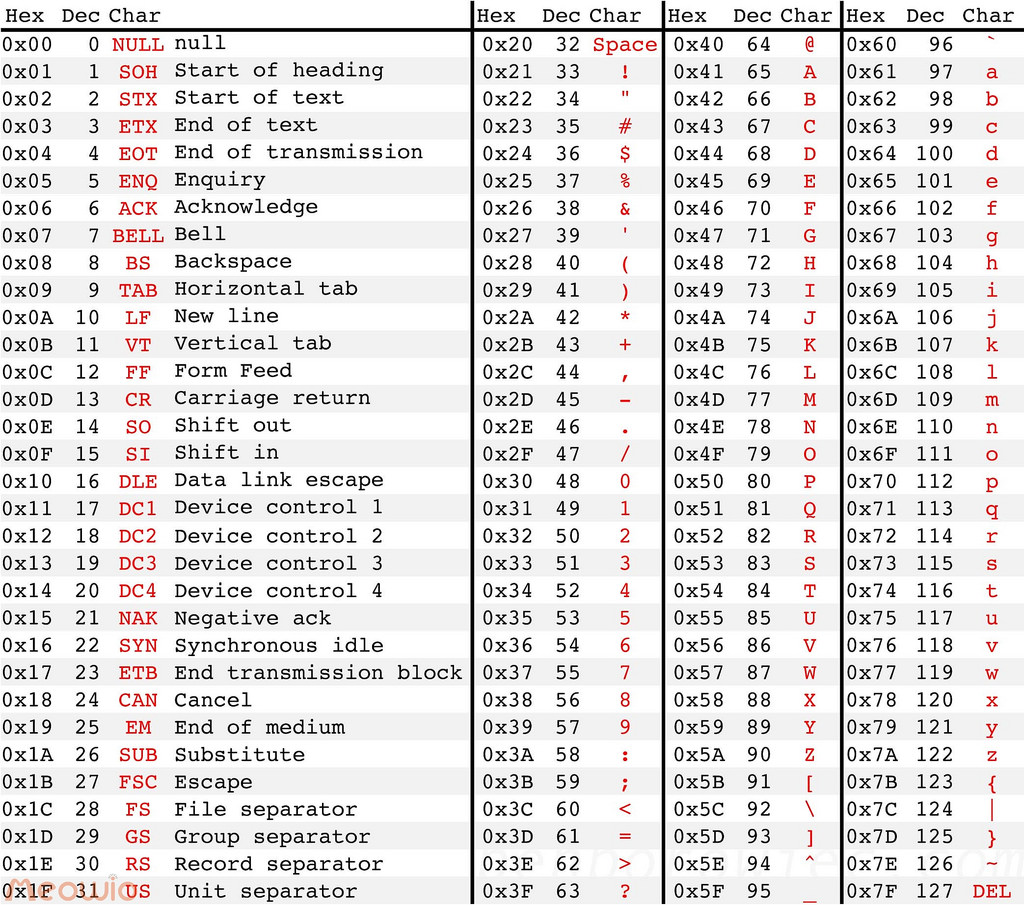
\includegraphics[width=0.65\textwidth]{figures/ascii.jpg}
\caption{\label{fig:ascii} \small An ASCII table, used in computer science for encoding text from standard input.}
\end{figure}
\end{frame}

\begin{frame}[fragile]{Hexadecimals, BCD, Gray-Codes, and ASCII}
\textbf{Example}: compiling the following C++ code on some machines still \textit{rings the bell}.
\begin{verbatim}
#include <stdio.h>
using namespace std;
int main()
{
char y = 7;
printf("%c\n",y);
return 0;
}
\end{verbatim}
\small
Often used in systems and code involving exchanging strings of text.
\end{frame}

\section{Conclusion}

\begin{frame}{Unit 1.3 Summary - Working with Binary}
\textbf{Reading: Digital Fundamentals (DF) Ch. 2 (see Moodle)}
\begin{enumerate}
\item Number representation
\item Binary conversions
\item Binary arithmetic
\item The floating-point system
\item Hexadecimals, Binary-Coded Decimals (BCD), Gray codes, and ASCII
\end{enumerate}
\textbf{Homework: exercises 5-16, 19-32, 35-38, 45, 53, 58 Ch. 2 (DF) (two weeks).}
\end{frame}

\end{document}
